\begin{frame}{Precision estimates at the LHC}
  \framesubtitle{Evidence for Beyond-Standard-Model physics}

  \begin{columns}

    \begin{column}{0.5\textwidth}

      \begin{figure}
        \centering
        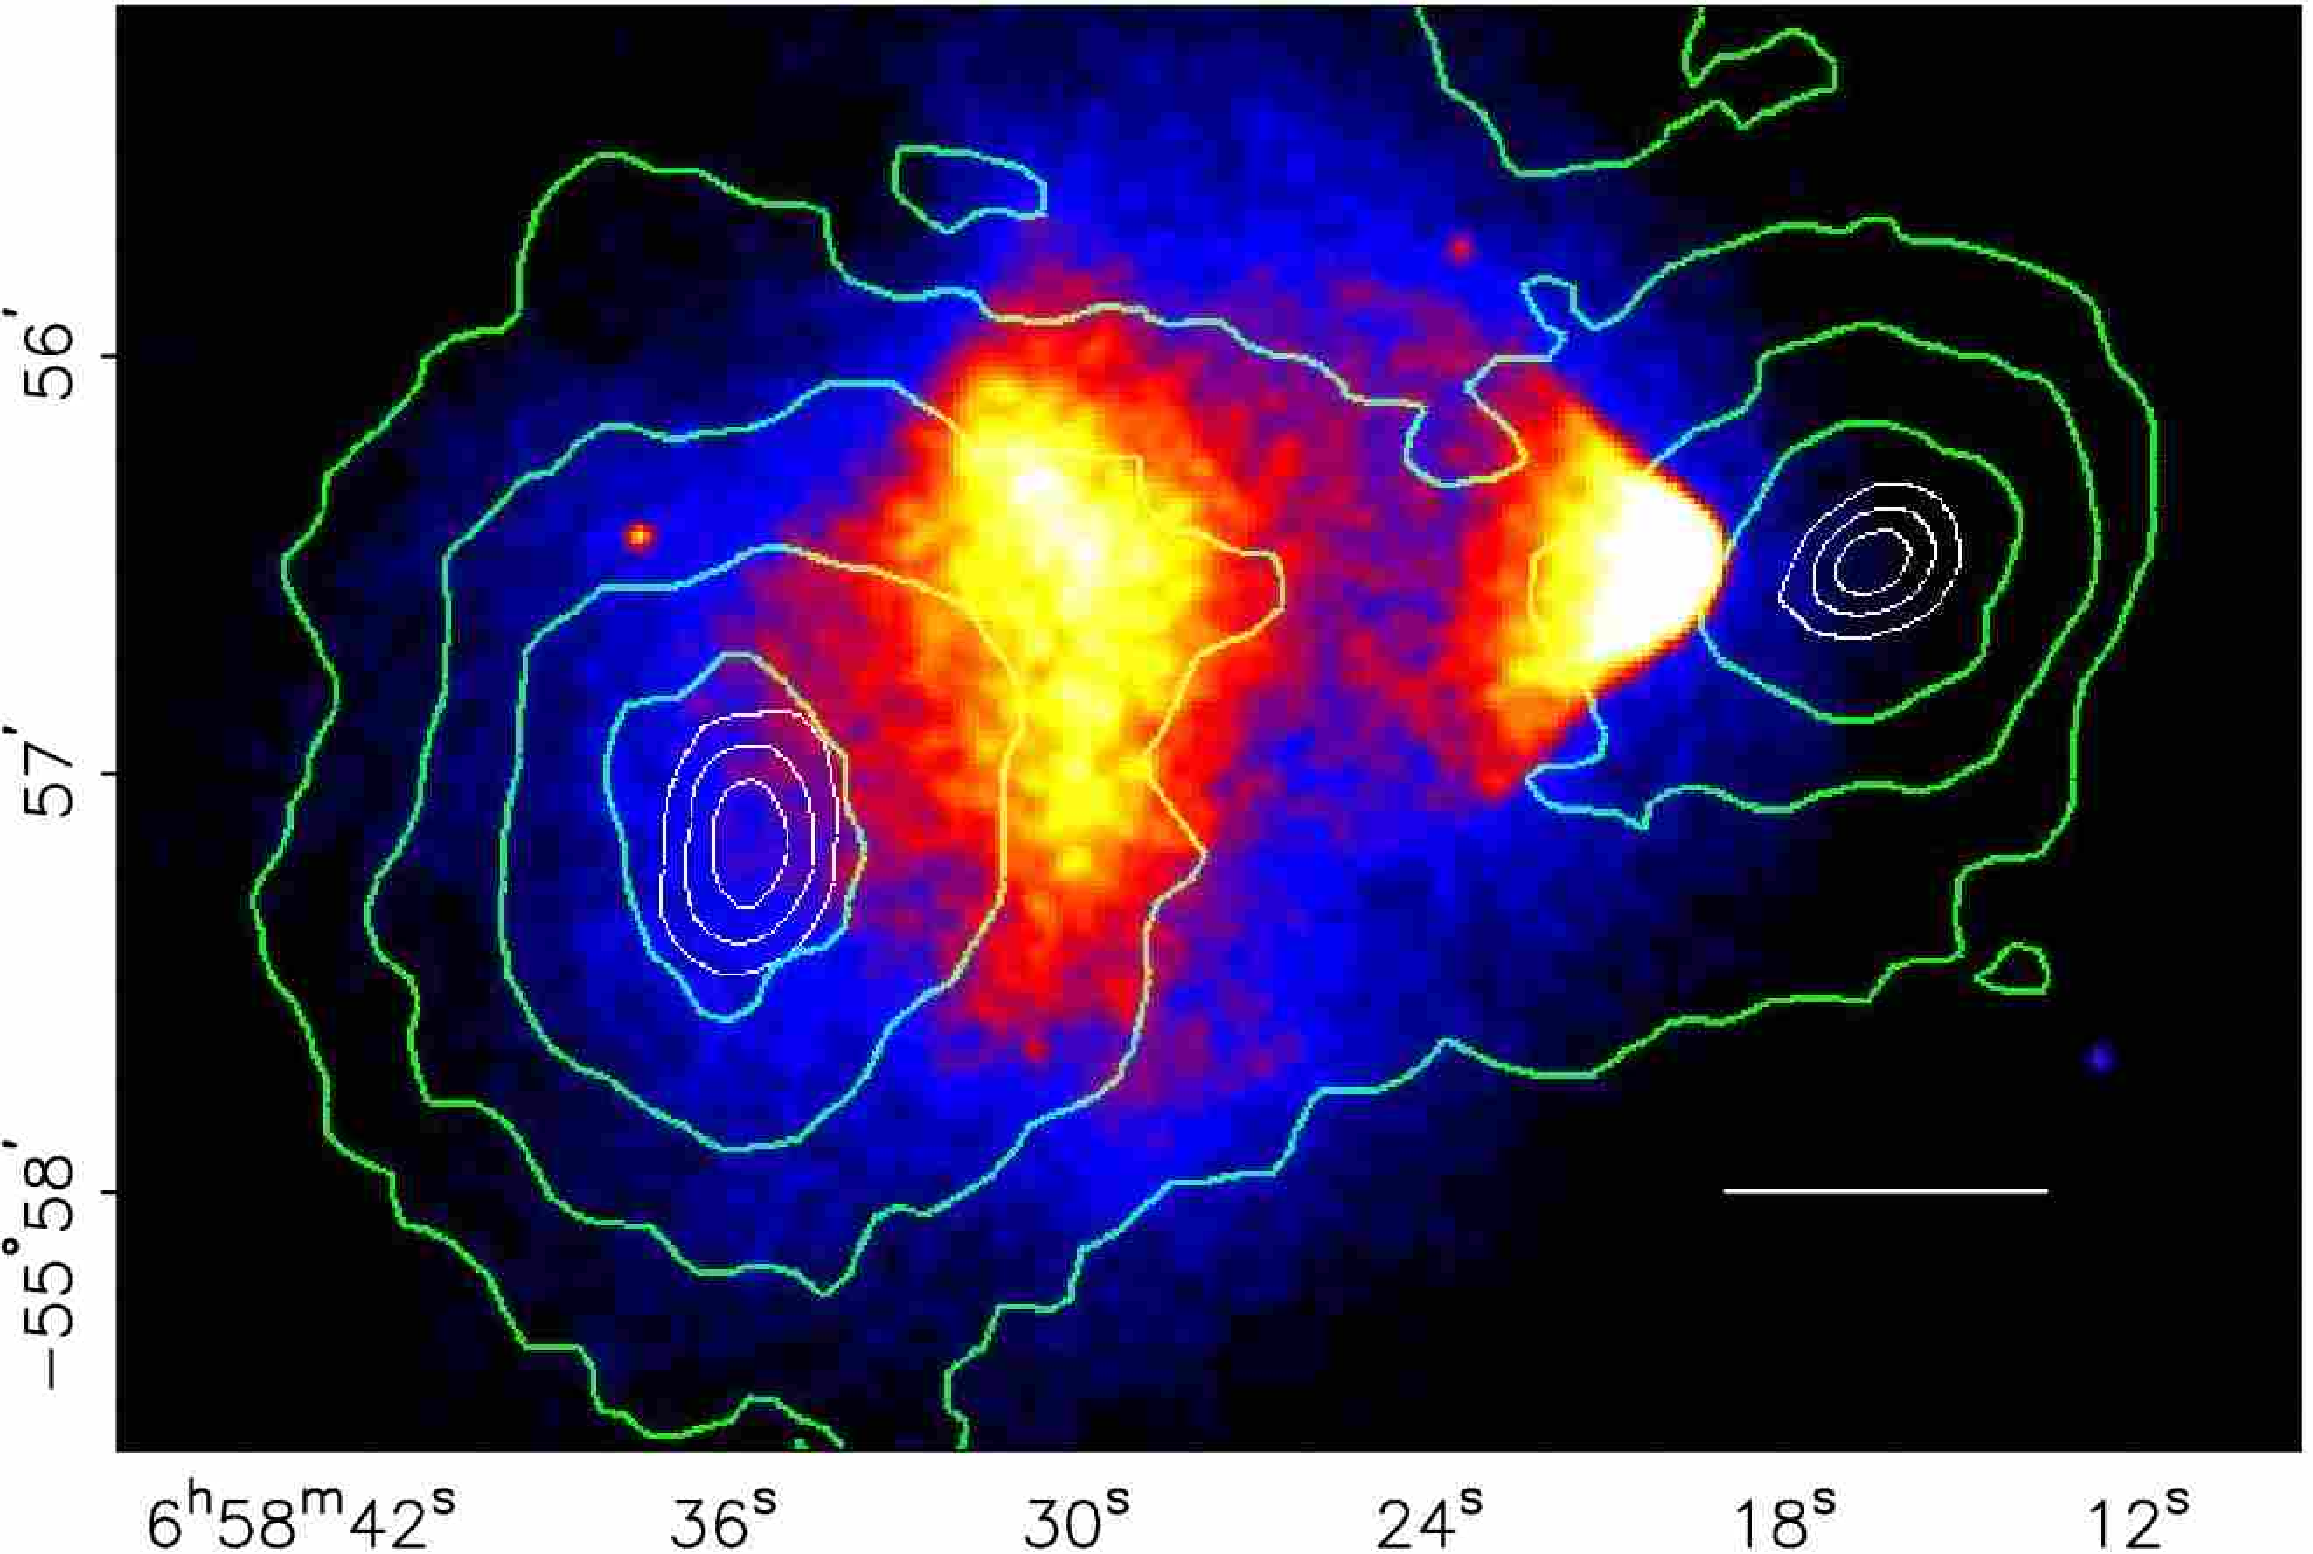
\includegraphics[width = \textwidth]{imgs/clowe-2.png}
      \end{figure}

    \end{column}

    \begin{column}{0.5 \textwidth}

      \begin{colorblock}[black]{statalegrey}{Main BSM evidence}
        \begin{itemize}
          \item dark matter and dark energy
          \item matter-antimatter asymmetry
          \item neutrino masses
        \end{itemize}
      \end{colorblock}

      \vspace{0.5em}


      \capcol{Figure} from Clowe et al. 2006.

      \justifying
      Offset between the observed baryonic mass distribution and the gravitational potential in the Bullet Cluster (1E 0657-56).

    \end{column}

  \end{columns}

\end{frame}

%=======================================================================

\begin{frame}{Precision estimates at the LHC}
  \framesubtitle{BSM constraints and shift in research paradigm}

  \begin{columns}

    \begin{column}{0.5 \textwidth}

      \begin{colorblock}[black]{statalegrey}{Main BSM proposals}
        \begin{itemize}
          \item supersymmetric models (MSSM, \dots)
          \item dark matter models (WIMPs, axions, \dots)
          \item extended gauge sectors ($ \mathrm{SO}(10) $, \dots)
          \item SM Effective Field Theory (SMEFT)
        \end{itemize}
      \end{colorblock}

      \vspace{0.5em}

      \capcol{Figure} from ATLA PUB Note 2023--025.

      \justifying
      Exclusion limits in the $ \tilde{g} - \tilde{\chi}^0_1 $ mass plane for various models for the decay of the gluino to the lightest supersymmetric particle.

    \end{column}

    \begin{column}{0.5\textwidth}

      \begin{figure}
        \centering
        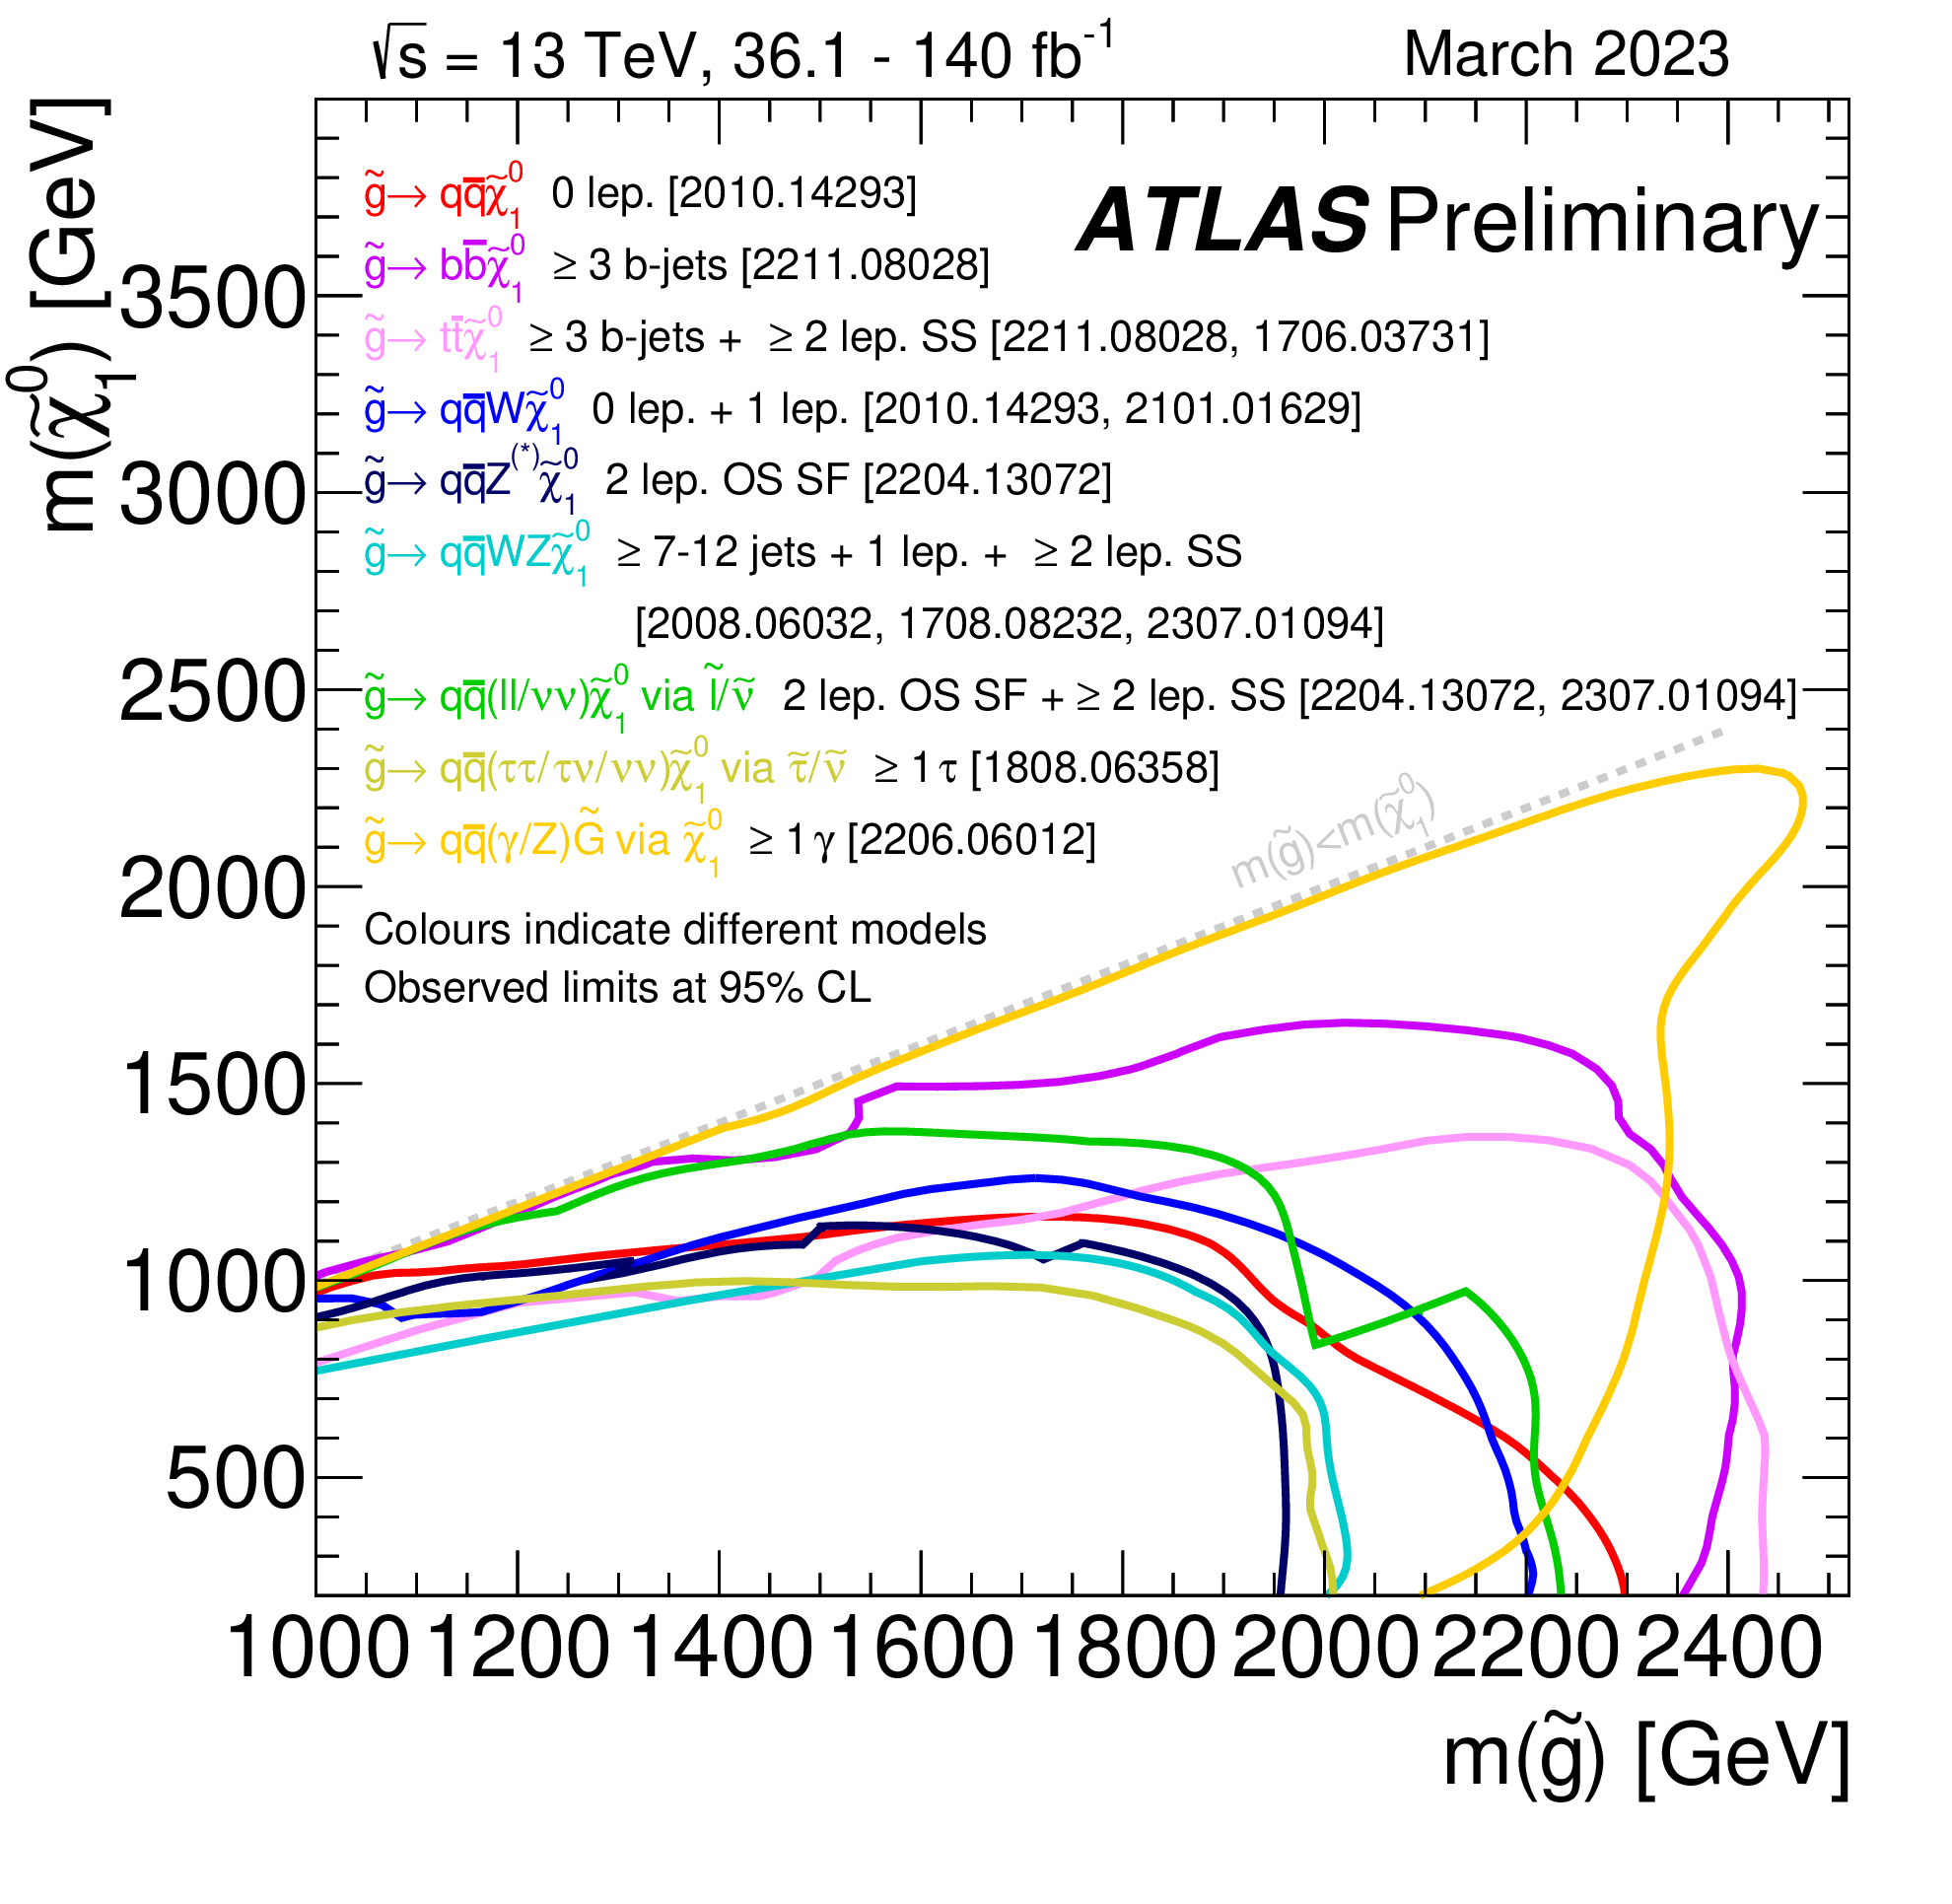
\includegraphics[width = 0.94\textwidth]{imgs/susy.png}
      \end{figure}

    \end{column}

  \end{columns}

\end{frame}

%=======================================================================

\begin{frame}{Precision estimates at the LHC}
  \framesubtitle{Factorization theorem and perturbative QCD}

  \begin{columns}

    \begin{column}{0.5 \textwidth}

      \begin{figure}
        \centering
        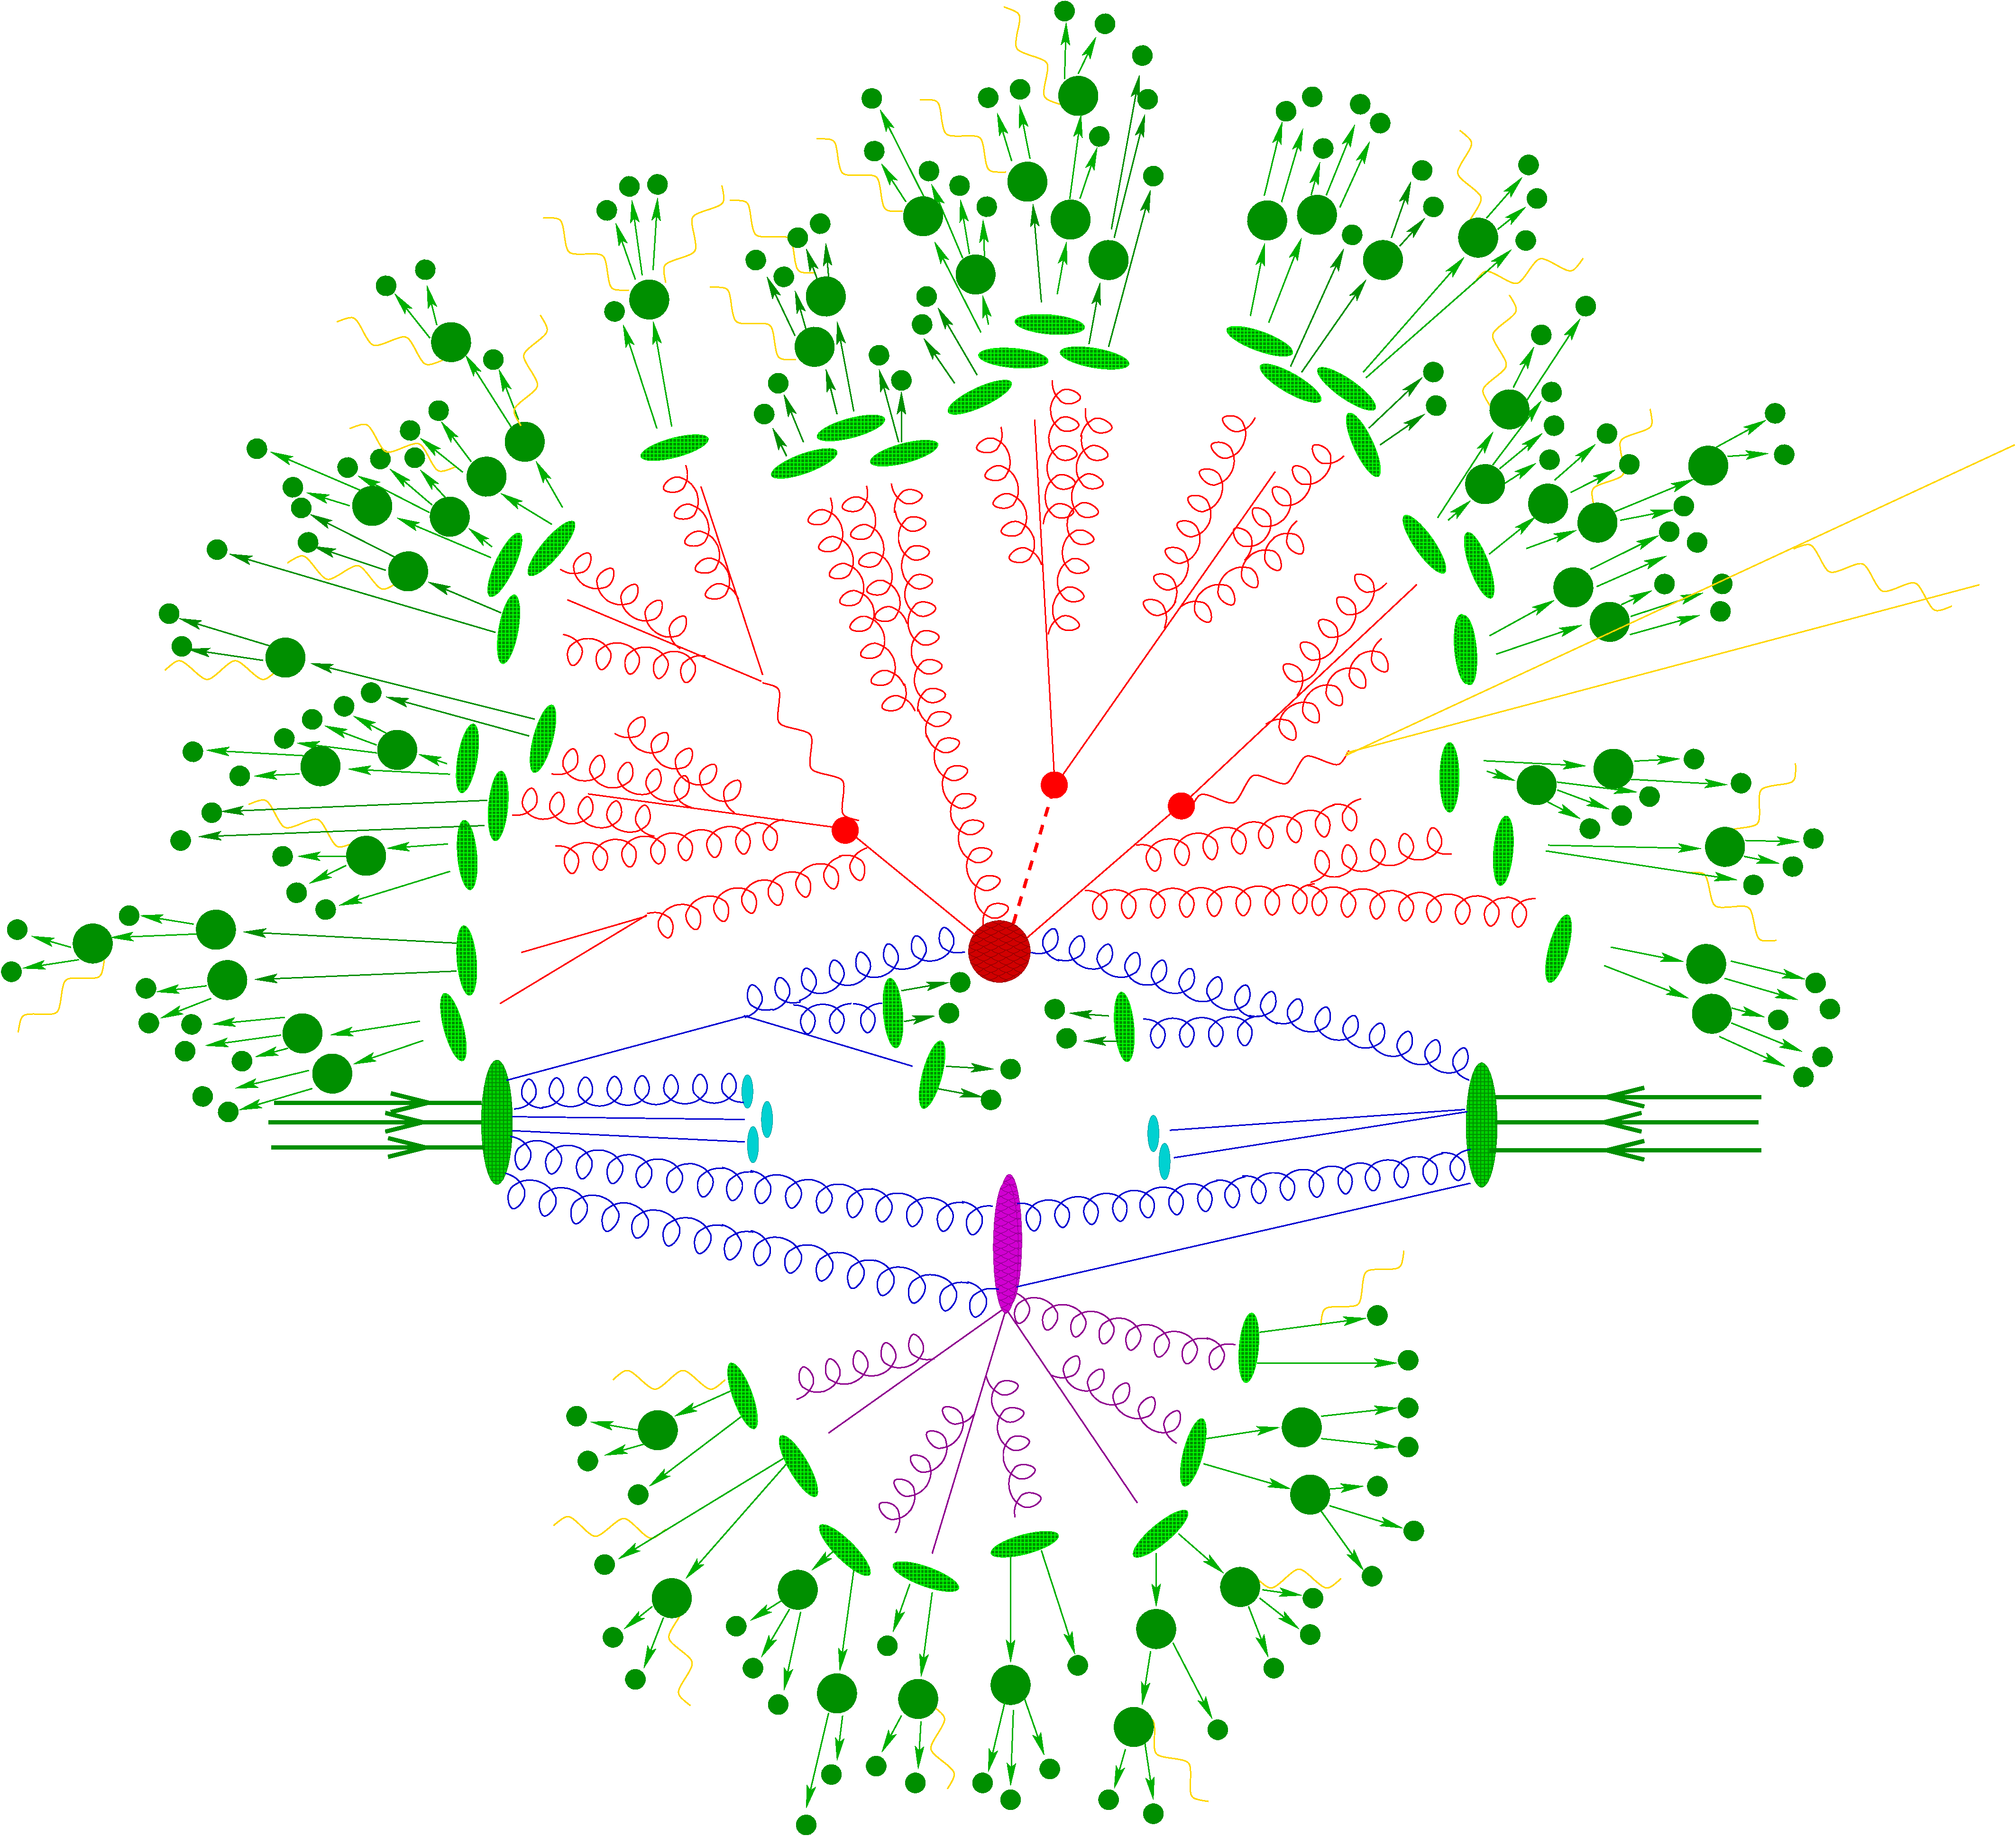
\includegraphics[width = \textwidth]{../imgs/hadr-scatt.pdf}
      \end{figure}

    \end{column}

    \begin{column}{0.5 \textwidth}

      \begin{figure}
        \centering
        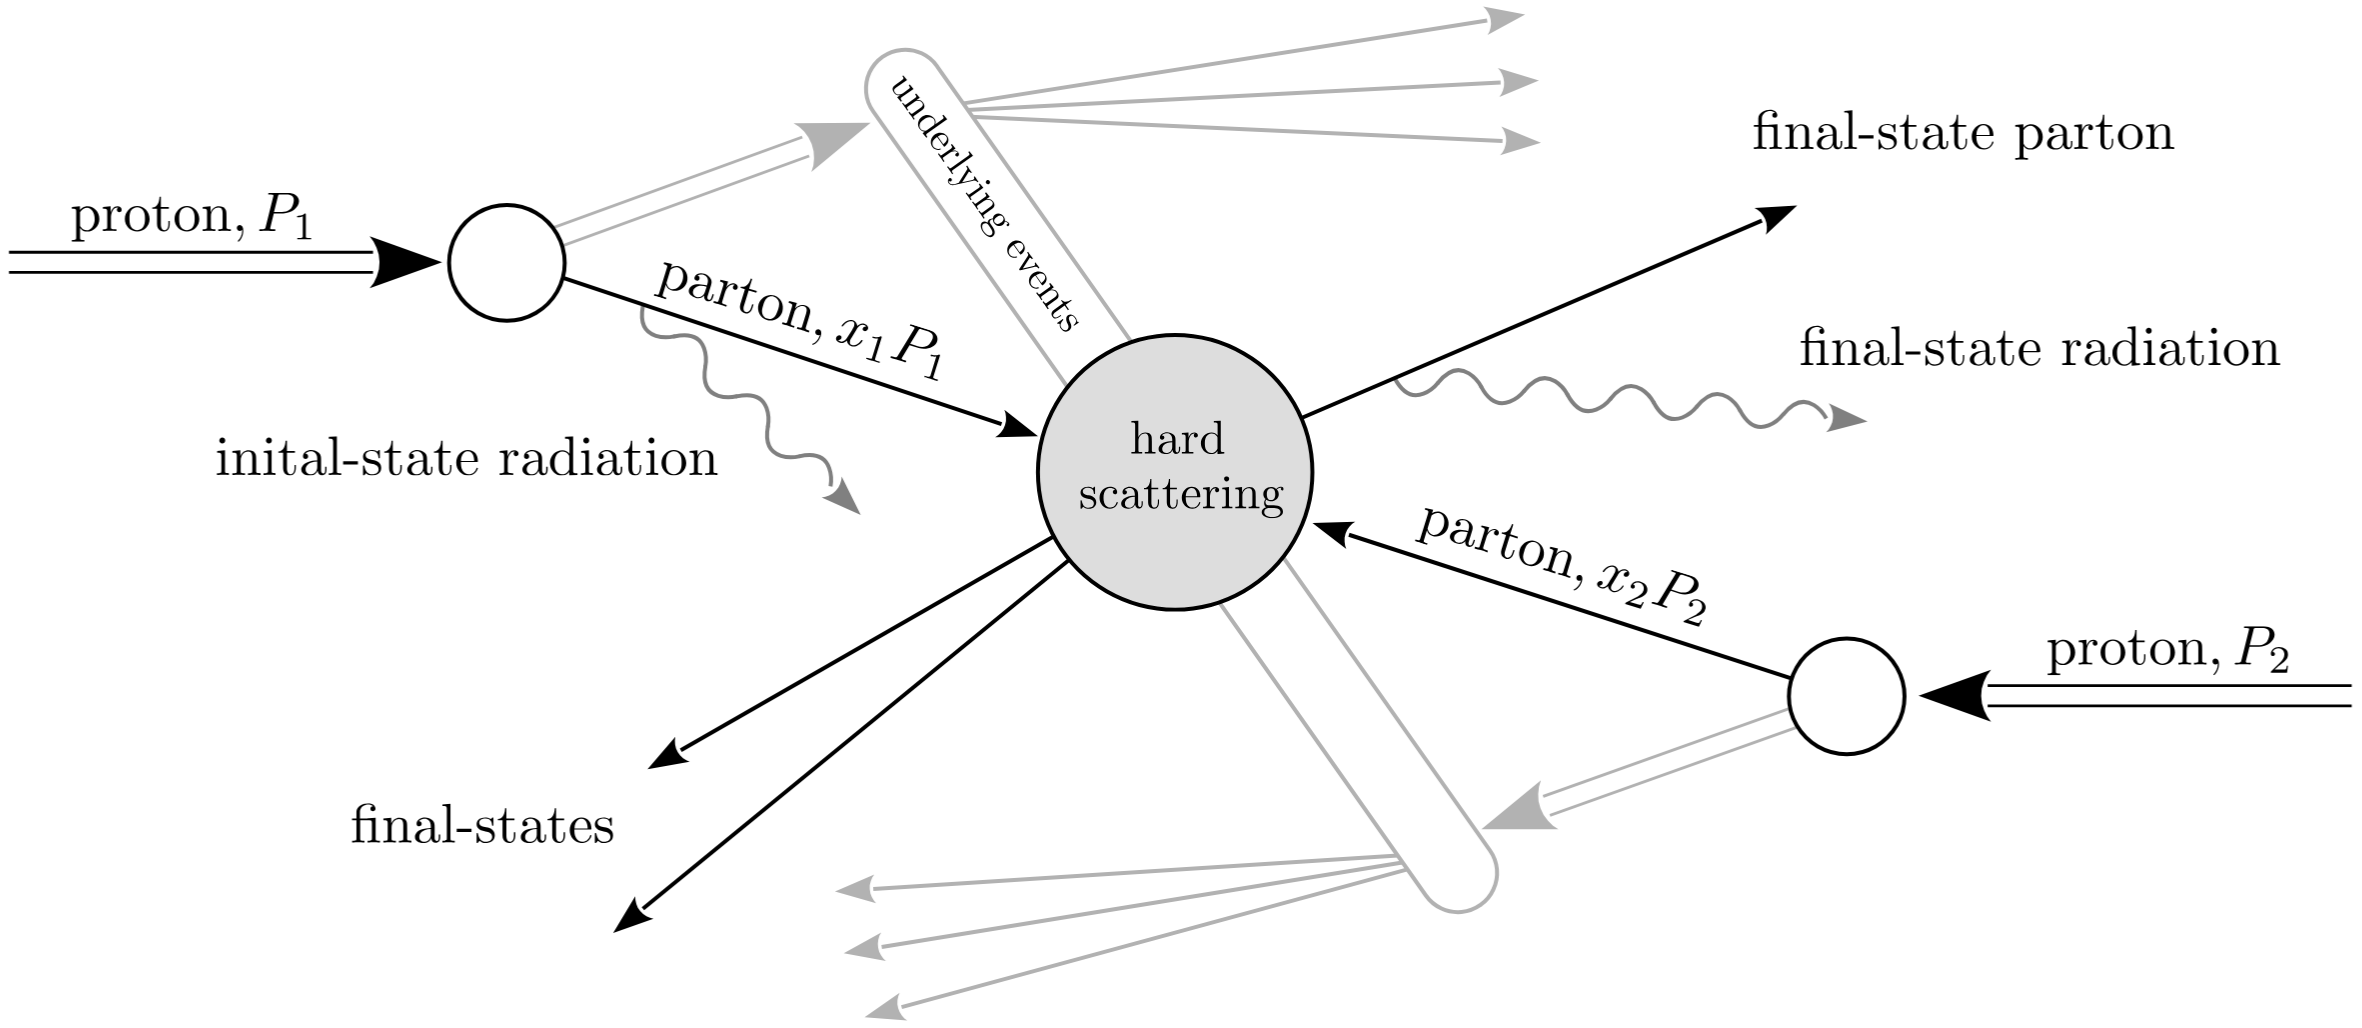
\includegraphics[width = \textwidth]{../imgs/part-scatt.png}
      \end{figure}

      \capcol{Figures} from Höche 2015 (left) and Asteriadis 2021 (right).

      \justifying
      Hadronization of jets produced in hadronic scattering and detail of the underlying hard partonic scattering.

    \end{column}

  \end{columns}

\end{frame}

%=======================================================================

\begin{frame}{Precision estimates at the LHC}
  \framesubtitle{Factorization theorem and perturbative QCD}

  \justifying
  Hadronic and partonic physics decouple in hard scattering processes, and we can formulate a factorization theorem:
  \begin{multline*}
    \dd\hcs_{h_1 , h_2}(P_1 , P_2) = \sum_{a,b} \int_{[0,1]^2} \frac{\dd \xi_1}{\xi_1} \frac{\dd \xi_2}{\xi_2} \,\pdfb{a}{h_1}(\xi_1, \fac^2) \,\pdfb{b}{h_2}(\xi_2, \fac^2) \times \\
    \times \dd\pcs_{a,b}(\xi_1 P_1, \xi_2 P_2, \rc, \ren^2, \fac^2)
    \left[ 1 + \smo \left( \frac{\qcd^n}{Q^n} \right) \right]
  \end{multline*}
  \emph{Asymptotic freedom} allows for a perturbative analysis of the hard partonic scattering:
  \begin{equation*}
    \dd\pcs_{a,b}(p_1 , p_2) = \sum_{n \in \N_0} \dd\pcs_{a,b}^{(n)}(p_1 , p_2)
  \end{equation*}
  $ n \ge 1 $ are denoted by N$ ^n $LO QCD corrections.

\end{frame}

%=======================================================================

\begin{frame}{IR-pole structure of QCD}
  \framesubtitle{Radiative corrections to partonic processes}

  \vspace{0.1em}

  Our focus is on NLO QCD corrections. Consider e.g. the Drell-Yan process:
  \begin{equation*}
    \begin{tikzpicture}
    \begin{feynman}

      \vertex (a1) {\(q\)};
      \vertex[below = 3cm of a1] (a2) {\(\bar{q}\)};

      \vertex[below = 1.5cm of a1] (b1) {};
      \vertex[right = 2.25cm of b1, dot] (v1) {};

      \vertex[right = 2.25cm of v1, dot] (v2) {};
      \vertex[right = 2.25cm of v2] (b2) {};

      \vertex[above = 1.5cm of b2] (a3) {$ \ell^- $};
      \vertex[below = 1.5cm of b2] (a4) {$ \ell^+ $};

      \diagram* {
	(a1) -- [fermion] (v1),
	(a2) -- [anti fermion] (v1),

        (v1) -- [photon, edge label = {$ \gamma^* / Z $}] (v2),

	(v2) -- [fermion] (a3),
	(v2) -- [anti fermion] (a4),
      };
    \end{feynman}
    \end{tikzpicture}
  \end{equation*}

  \centering
  LO process

\end{frame}

%=======================================================================

\begin{frame}[noframenumbering]{IR-pole structure of QCD}
  \framesubtitle{Radiative corrections to partonic processes}

  Our focus is on NLO QCD corrections. Consider e.g. the Drell-Yan process:
  \begin{equation*}
    \begin{tikzpicture}
    \begin{feynman}

      \vertex (a1) {\(q\)};
      \vertex[below = 3cm of a1] (a2) {\(\bar{q}\)};

      \vertex[below = 1.5cm of a1] (b1) {};
      \vertex[right = 2.25cm of b1, dot] (v1) {};

      \vertex[right = 2.25cm of v1, dot] (v2) {};
      \vertex[right = 2.25cm of v2] (b2) {};

      \vertex[above = 1.5cm of b2] (a3) {$ \ell^- $};
      \vertex[below = 1.5cm of b2] (a4) {$ \ell^+ $};

      \vertex[dot , red] (c1) at ($(a1) + (1.5,-1)$) {};
      \vertex (c2) at ($(c1) + (1.5,1)$) {\color{red} $ g $};

      \diagram* {
	(a1) -- [fermion] (v1),
	(a2) -- [anti fermion] (v1),

        (v1) -- [photon, edge label = {$ \gamma^* / Z $}] (v2),

	(v2) -- [fermion] (a3),
	(v2) -- [anti fermion] (a4),

	(c1) -- [gluon, red] (c2),
      };
    \end{feynman}
    \end{tikzpicture}
  \end{equation*}

  \centering
  \color{red} Real correction

\end{frame}

%=======================================================================

\begin{frame}[noframenumbering]{IR-pole structure of QCD}
  \framesubtitle{Radiative corrections to partonic processes}

  Our focus is on NLO QCD corrections. Consider e.g. the Drell-Yan process:
  \begin{equation*}
    \begin{tikzpicture}
    \begin{feynman}

      \vertex (a1) {\(q\)};
      \vertex[below = 3cm of a1] (a2) {\(\bar{q}\)};

      \vertex[below = 1.5cm of a1] (b1) {};
      \vertex[right = 2.25cm of b1, dot] (v1) {};

      \vertex[right = 2.25cm of v1, dot] (v2) {};
      \vertex[right = 2.25cm of v2] (b2) {};

      \vertex[above = 1.5cm of b2] (a3) {$ \ell^- $};
      \vertex[below = 1.5cm of b2] (a4) {$ \ell^+ $};

      \vertex[dot, blue] (c1) at ($(a1) + (0.75,-0.5)$) {};
      \vertex[dot, blue] (c2) at ($(a2) + (0.75,0.5)$) {};

      \diagram* {
	(a1) -- [fermion] (v1),
	(a2) -- [anti fermion] (v1),

        (v1) -- [photon, edge label = {$ \gamma^* / Z $}] (v2),

	(v2) -- [fermion] (a3),
	(v2) -- [anti fermion] (a4),

      (c1) -- [gluon, bend right, edge label' = {$ g^* $}, blue] (c2),
      };
    \end{feynman}
    \end{tikzpicture}
  \end{equation*}

  \centering
  \color{blue} Virtual correction

\end{frame}

%=======================================================================

\begin{frame}{IR-pole structure of QCD}
  \framesubtitle{Infrared singularities of scattering amplitudes}

  Main difficulty: infrared singularities in particular kinematic regimes.

  \vspace{-0.01em}

  Example in real corrections:

  \begin{equation*}
  \begin{tikzpicture}[baseline = (r.base)]
    \begin{feynman}[inline = (r.base)]
      \vertex (a);
      \vertex[right = 2.5cm of a, dot] (b) {};
      \vertex[right = 2.5cm of b, blob, minimum size = 1.2cm] (c) {};

      \vertex[above = 1.5cm of b] (d);
      \vertex[right = 1.5cm of d] (e);

      \vertex[below = 0.25em of b] (r);

      \diagram* {
	(a) -- [fermion, momentum' = \(p\)] (b),
	(b) -- [fermion, momentum' = \(p - k\)] (c),

	(b) -- [gluon, momentum = \(k\)] (e),
      };
    \end{feynman}
  \end{tikzpicture}
  \quad \sim \quad
  \frac{1}{(p - k)^2} = - \frac{1}{2 E_p E_k ( 1 - \cos \theta )}
  \end{equation*}

  \vspace{0.91em}

\end{frame}

%=======================================================================

\begin{frame}[noframenumbering]{IR-pole structure of QCD}
  \framesubtitle{Infrared singularities of scattering amplitudes}

  Main difficulty: infrared singularities in particular kinematic regimes.

  Example in real corrections:

  \begin{equation*}
  \begin{tikzpicture}[baseline = (r.base)]
    \begin{feynman}[inline = (r.base)]
      \vertex (a);
      \vertex[right = 2.5cm of a, dot] (b) {};
      \vertex[right = 2.5cm of b, blob, minimum size = 1.2cm] (c) {};

      \vertex[above = 1.5cm of b] (d);
      \vertex[right = 1.5cm of d] (e);

      \vertex[below = 0.25em of b] (r);

      \diagram* {
	(a) -- [fermion, momentum' = \(p\)] (b),
	(b) -- [fermion, momentum' = \(p - k\)] (c),

	(b) -- [gluon, momentum = \(k\)] (e),
      };
    \end{feynman}
  \end{tikzpicture}
  \quad \sim \quad
  \frac{1}{(p - k)^2} = - \frac{1}{2 E_p \textcolor{red}{E_k} ( 1 - \cos \theta )}
  \end{equation*}

  \centering
  \color{red} Soft singularity: $ E_k \rightarrow 0 $

\end{frame}

%=======================================================================

\begin{frame}[noframenumbering]{IR-pole structure of QCD}
  \framesubtitle{Infrared singularities of scattering amplitudes}

  Main difficulty: infrared singularities in particular kinematic regimes.

  Example in real corrections:

  \begin{equation*}
  \begin{tikzpicture}[baseline = (r.base)]
    \begin{feynman}[inline = (r.base)]
      \vertex (a);
      \vertex[right = 2.5cm of a, dot] (b) {};
      \vertex[right = 2.5cm of b, blob, minimum size = 1.2cm] (c) {};

      \vertex[above = 1.5cm of b] (d);
      \vertex[right = 1.5cm of d] (e);

      \vertex[below = 0.25em of b] (r);

      \diagram* {
	(a) -- [fermion, momentum' = \(p\)] (b),
	(b) -- [fermion, momentum' = \(p - k\)] (c),

	(b) -- [gluon, momentum = \(k\)] (e),
      };
    \end{feynman}
  \end{tikzpicture}
  \quad \sim \quad
  \frac{1}{(p - k)^2} = - \frac{1}{2 E_p E_k \textcolor{blue}{( 1 - \cos \theta )}}
  \end{equation*}

  \centering
  \color{blue} Collinear singularity: $ \theta \rightarrow 0 $

\end{frame}

%=======================================================================

\begin{frame}{IR-pole structure of QCD}
  \framesubtitle{Dimensional regularization}

  The key idea to regularize IR divergences is dimensional regularization:
  \vspace{-0.01em}
  \begin{equation*}
    d = 4 - 2 \de
    \quad , \quad
    \de \in \C : \Re{\de} < 0
  \end{equation*}
  Then, soft and collinear singularities are expressed as poles in $ \de $:
  \begin{equation*}
    \int \frac{\dd^{d-1}k}{(2\pi)^{d-1} 2E_k} \abs{\ampl(p_k)}^2 \sim \int_0^{\ema} \frac{\dd E_k}{E_k^{5-d}} \int_0^\pi \dd \theta \frac{\sin^{d-3} \theta}{1 - \cos \theta} \abs{\ampl_0}^2
  \end{equation*}

  \vspace{2.81em}

\end{frame}

%=======================================================================

\begin{frame}{IR-pole structure of QCD}
  \framesubtitle{Dimensional regularization}

  The key idea to regularize IR divergences is dimensional regularization:
  \begin{equation*}
    d = 4 - 2 \de
    \quad , \quad
    \de \in \C : \Re{\de} < 0
  \end{equation*}
  Then, soft and collinear singularities are expressed as poles in $ \de $:
  \begin{equation*}
    \begin{split}
      \int \frac{\dd^{d-1}k}{(2\pi)^{d-1} 2E_k} \abs{\ampl(p_k)}^2 \sim
      & \, \textcolor{red}{\int_0^{\ema} \frac{\dd E_k}{E_k^{5-d}}} \int_0^\pi \dd \theta \frac{\sin^{d-3} \theta}{1 - \cos \theta} \abs{\ampl_0}^2 \\
      \begin{array}{r}
        \textcolor{red}{\text{soft singularity}} \\
        \text{ }
      \end{array}
      & \textcolor{red}{= - \frac{\ema^{-2\de}}{2\de}}
    \end{split}
  \end{equation*}

\end{frame}

%=======================================================================

\begin{frame}{IR-pole structure of QCD}
  \framesubtitle{Dimensional regularization}

  The key idea to regularize IR divergences is dimensional regularization:
  \begin{equation*}
    d = 4 - 2 \de
    \quad , \quad
    \de \in \C : \Re{\de} < 0
  \end{equation*}
  Then, soft and collinear singularities are expressed as poles in $ \de $:
  \begin{equation*}
    \begin{split}
      \int \frac{\dd^{d-1}k}{(2\pi)^{d-1} 2E_k} \abs{\ampl(p_k)}^2 \sim
      & \, \textcolor{red}{\int_0^{\ema} \frac{\dd E_k}{E_k^{5-d}}} \, \textcolor{blue}{\int_0^\pi \dd \theta \frac{\sin^{d-3} \theta}{1 - \cos \theta}} \abs{\ampl_0}^2 \\
      \begin{array}{r}
        \textcolor{red}{\text{soft singularity}} \\
        \textcolor{blue}{\text{collinear singularity}}
      \end{array}
      & \textcolor{red}{= - \frac{\ema^{-2\de}}{2\de}} \quad \textcolor{blue}{= - \frac{2^{-2 + \de}}{\de}}
    \end{split}
  \end{equation*}

\end{frame}

%=======================================================================

\begin{frame}{IR-pole structure of QCD}
  \framesubtitle{Subtraction schemes}

  $ \de $-poles can be extracted from partonic cross-sections via subtraction methods.

  General idea using a regular function $ f(x) $:
  \begin{equation*}
    I = \int_0^1 \frac{\dd x}{x^{1 + \de}} \,f(x) = \int_0^1 \frac{\dd x}{x^{1 + \de}} \left[ \,f(x) - f(0) \right] + f(0) \int_0^1 \frac{\dd x}{x^{1 + \de}}
  \end{equation*}
  \begin{itemize}
    \item $ \displaystyle \frac{\,f(x) - f(0)}{x^{1 + \de}} $ regular at $ x = 0 $, so it can be numerically integrated with $ \de \rightarrow 0 $
    \item $ \displaystyle f(0) \int_0^1 \frac{\dd x}{x^{1 + \de}} = - \frac{\,f(0)}{\de} $ contains the explicit $ \de $-pole
  \end{itemize}

  Our aim is finding the most general subtraction terms $ \,f(0) $ for partonic scattering.

\end{frame}

%=======================================================================

\begin{frame}{NSC subtraction scheme}
  \framesubtitle{Extraction of poles via operators}

  introduce the NSC SS

\end{frame}

%=======================================================================

\begin{frame}{NSC subtraction scheme}
  \framesubtitle{Pole cancellation}

  briefly show pole cancellation in the NSC SS

\end{frame}

%=======================================================================

\begin{frame}{NSC SS with massive quarks}
  \framesubtitle{Mass-regualtion of soft and collinear limits}

  explain why massive quarks change $ I_\text{S}(\epsilon) $ and $ I_\text{V}(\epsilon) $, but not $ I_\text{C}(\epsilon) $

\end{frame}

%=======================================================================

\begin{frame}{NSC SS with massive quarks}
  \framesubtitle{Generalized soft operator}

  show how $ I_\text{S}(\epsilon) $ changes (in particular massive angular integrals)

\end{frame}

%=======================================================================

\begin{frame}{NSC SS with massive quarks}
  \framesubtitle{Generalized virtual operator}

  show how $ I_\text{V}(\epsilon) $ changes (in particular, colour-correlated $ \epsilon^{-2} $-poles in $ \mathcal{V}_{i,j}(\epsilon) $ coefficients)

\end{frame}

%=======================================================================

\begin{frame}{NSC SS with massive quarks}
  \framesubtitle{Pole cancellation: generalized pole terms}

  highlights of pole cancellation in $ I_{\text{S}+\text{V}}(\epsilon) $, define $ \chi_{i,j}(\epsilon) $ coefficients and explain their property

\end{frame}

%=======================================================================

\begin{frame}{NSC SS with massive quarks}
  \framesubtitle{Pole cancellation: colour-correlated terms}

  show pole cancellation in the colour-correlated sum of $ I_{\text{S}+\text{V}}(\epsilon) $, leaving the same (and opposite) pole terms of $ I_\text{C}(\epsilon) $

\end{frame}

%=======================================================================

\begin{frame}{NSC SS with massive quarks}
  \framesubtitle{Generalized integrated counterterms}

  show integrated counterterms and highlighting massive logs

\end{frame}


%=======================================================================

\begin{frame}{Conclusions}
  \framesubtitle{Future developments}

  draw conclusions and point out possible further developments

\end{frame}










